\subsection{مقدمه}
\subsubsection{نصب MySQL}
برای نصب
\lr{MySQL}
من از
\link{https://www.digitalocean.com/community/tutorials/how-to-install-mysql-on-ubuntu-20-04}{این}
راهنما استفاده کردیم. به صورت خیلی خلاصه ما از خود
\lr{apt} ورژن \lr{8.0.33}
را نصب کردیم. این مراحل را برای نصب در ماشین مجازی و حقیقی انجام دادیم.
\subsubsection{تنظیم HammerDB}
تنظیم
\lr{HammerDB}
تا مقدار بسیار خوبی شبیه
\lr{PostgreSQL}
است ولی با این تفاوت که یک فیلد به اسم
\lr{MySQL Socket}
نیز به
\lr{HammerDB}
اضافه شده است. این مقدار باید برابر با
\lr{unix socket}ای
باشد که
\lr{MySQL}
بر روی کامپیوتر باز می‌کند که به نسبت
\lr{TCP/IP}
سریع‌تر باشد. در صورتی که مقدار
\codeword{null} % https://www.hammerdb.com/docs/ch04s03.html
را در این فیلد وارد کنیم
\lr{HammerDB}
فورس می‌شود که از
\lr{TCP/IP}
به جای
\lr{unix socket}
استفاده کند. این کار برای وصل شدن به ماشین مجازی لازم است چرا که به
\lr{unix socket}های
داخل ماشین مجازی دسترسی نداریم. بقیه‌ی مراحل ساخت
\lr{schema}
و خود تست مانند
\lr{PostgreSQL}
است و تفاوتی ندارد. نمونه‌ای از تنظیمات
\lr{MySQL} در \lr{HammerDB}
را می‌توانید در شکل
\ref{fig:mysql:init:hammerdb_driver}
مشاهده کنید. همچنین در صورتی که بخواهید از مسیر
\lr{MySQL unix socket}
مطلع شوید می‌توانید آن را به کمک دستور
\codeword{SELECT @@SOCKET}
در
\lr{MySQL}
مانند شکل
\ref{fig:mysql:init:unixsocket}
مشاهده کنید.
\begin{figure}[H]
    \centering
    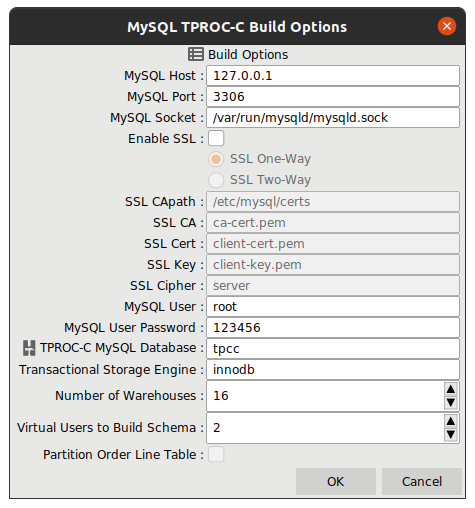
\includegraphics[scale=0.5]{pictures/mysql/baremetal/hammerdb-driver.png}
    \caption{تنظیمات \lr{MySQL} در \lr{HammerDB}}
    \label{fig:mysql:init:hammerdb_driver}
\end{figure}
\begin{figure}[H]
    \centering
    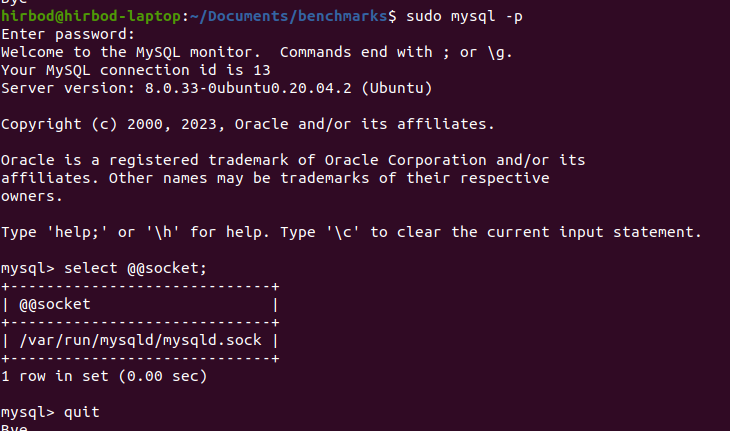
\includegraphics[scale=0.5]{pictures/mysql/baremetal/socket-path.png}
    \caption{مسیر \lr{unix socket} در \lr{MySQL}}
    \label{fig:mysql:init:unixsocket}
\end{figure}
\subsubsection{تنظیم MySQL در VM}
مانند
\lr{PostgreSQL}،
برای اینکه بتوانیم از
\lr{host}
به
\lr{VM}
وصل شویم باید
\lr{IP}های
مجاز برای وصل شدن به هر کاربر را مشخص کنیم. اما در ابتدا باید به
\lr{MySQL}
بگوییم که بر روی تمامی
\lr{interface}ها \lr{listen}
کند چرا که به صورت پیشفرض فقط بر روی
\lr{localhost}
کار می‌کند. برای این کار باید فایل
\codeword{/etc/mysql/mysql.d/my.cnf}
را عوض کنیم و در قسمت
\codeword{[mysqld]}
خط زیر را اضافه یا عوض کنیم:
\codebox{bind-address=0.0.0.0}
در ادامه نیز باید کابری بسازیم که اجازه‌ی اتصال از تمامی
\lr{IP}ها را داشته باشد.
برای این کار از دستورات زیر در ترمینال
\lr{MySQL}
استفاده می‌کنیم:
\codebox{
    CREATE USER 'hirbod'@'\%' IDENTIFIED BY '123456';\\
    GRANT ALL PRIVILEGES ON *.* TO 'hirbod'@'\%' WITH GRANT OPTION;\\
    FLUSH PRIVILEGES;
}
بعد از این دستورات، مانند شکل
\ref{fig:mysql:init:host_to_vm}
می‌توان از
\lr{host} به \lr{guest}
وصل شد.
\begin{figure}[H]
    \centering
    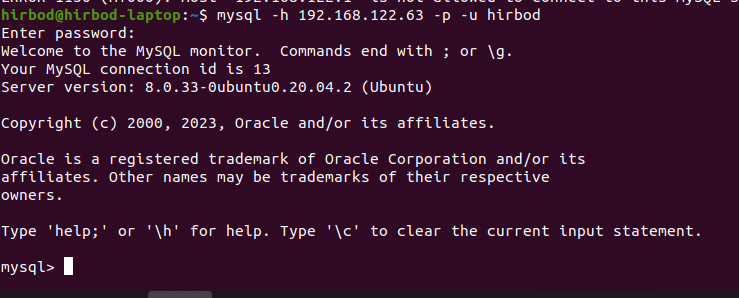
\includegraphics[scale=0.5]{pictures/mysql/vm/connection.png}
    \caption{وصل شدن به \lr{MySQL} از \lr{host} به \lr{guest}}
    \label{fig:mysql:init:host_to_vm}
\end{figure}
\subsubsection{اسپم شدن strace}
یکی از مشکلات عجیبی که در
\lr{MySQL}
به وجود آمد زمانی بود که می‌خواستیم
\lr{strace}
بگیریم. اول از همه اینکه
\codeword{-f}
را یادم رفته بود برای همین کلا لاگ خالی بود! اما بعد از زدن
\codeword{-f}
در دستور
\lr{perf}
متوجه شدم که فایل خروجی بسیار بزرگ است و مثلا برای یک ران 3 دقیقه‌ای حدود 5 گیگابایت فایل درست شده بود!
بعد از نگاه کردن به لاگ‌ها متوجه شدم که
\lr{MySQL}
زمان بسیار زیادی را صرف استفاده از
\link{https://man7.org/linux/man-pages/man2/futex.2.html}{futex}
و
\link{https://man7.org/linux/man-pages/man2/io_getevents.2.html}{io\_getevents}
می‌کند. به همین منظور در
\lr{strace}
این دو
\lr{syscall} را \lr{exclude}
کردیم که در لاگ‌ها نیاییند.

\textbf{پی‌نوشت:} برای من سوال شد که چرا حتی زمانی که \lr{MySQL} در حالت \lr{idle}
است در حال استفاده از این دو
\lr{syscall}
است؟ کمی به نظر شما عجیب نیست این موضوع و جای بحث و تحقیق بیشتر ندارد؟